\noindent 
In this project, we envision to develop a PIM system depicted in Figure~\ref{fig:arch}. 
Overall, the system consists of a 16-node accelerator-memory (AM) cluster and IBM POWER8-based host systems.
 
An AM cluster is comprised of 16 nodes (packages) connected by our power-efficient high-bandwidth chip-to-chip links in a mesh style. 
One accelerator (ACC) and four 8GB DiRAM4 dies will constitute a PIM package with 4TB/s aggregate in-package bandwidth. 
Our ACC die will integrate 32 ACCs with our custom eDRAM, a 32×32 crossbar, and a network interface (NI) to support chip-to-chip communications.

\begin{wrapfigure}{r}[0pt]{0.6\textwidth}
\center
%\vspace{-8ex}
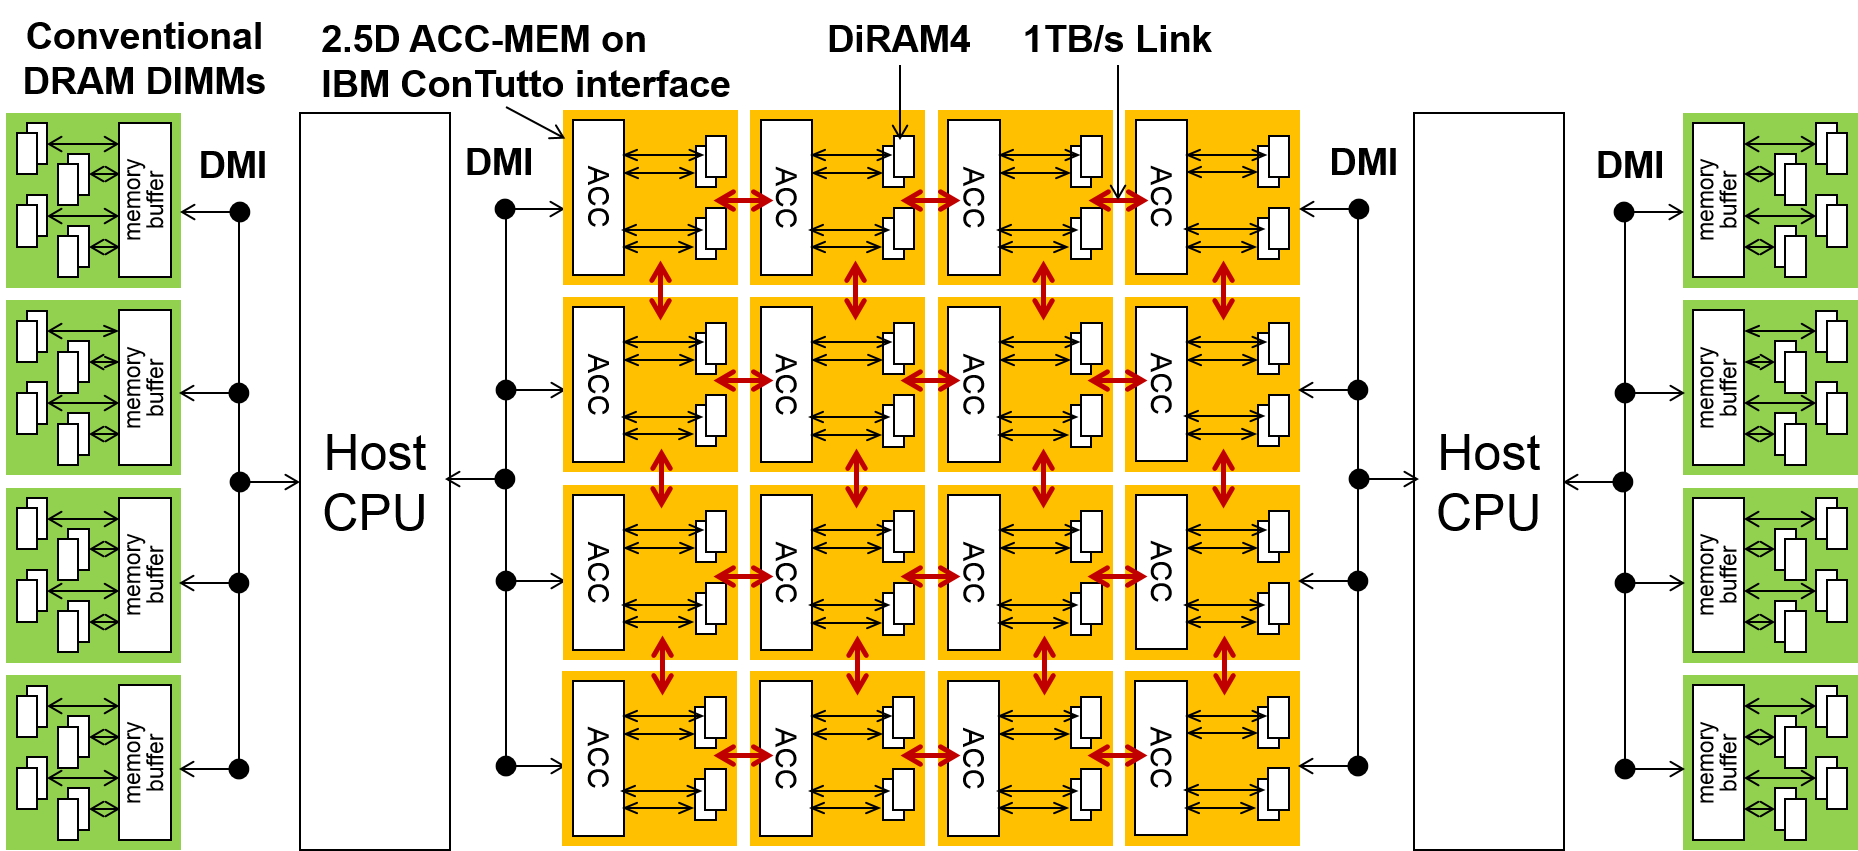
\includegraphics[width=1.0\linewidth]{./fig/arch.png}
\caption{The overall architecture of an Accelerator-Memory HIVE.}
\label{fig:arch}
\end{wrapfigure}

In the proposed PIM system, we propose to connect each AM packages to a memory channel of a host CPU providing 8 memory channels;
the memory channel provides the highest bandwidth with the lowest latency amongst off-chip communication interfaces in contemporary computer systems.
A IBM's ConTutto module facilitates the interface between an AM package and the IBM's proprietary memory interface (DMI).
The memory space associated with the AM cluster is a non-cacheable region to eliminate the need for managing cache coherence between caches of the host systems and the AM HIVE.
The host system allocates the memory space of the AM cluster as a sinlge, continuous, and large physical memory segment which is preferred by big-data applications~\footnote{}.
ACCs are memory-mapped to part of the non-cacheable regions (as other I/O devices).

% Some notes
% We need a custom POWER8 board
